\documentclass[titlepage,oneside,11pt]{book}
\author{Nikita Belyavskij}
% Need to add subtitle
\title{EFL Edje Theme Editor}

\usepackage{xcolor,graphicx}
%\usepackage[pdftex]{hyperref}
\begin{document}
% generates the title
\maketitle
% insert the table of contents
\tableofcontents
\chapter{Introduction}
%This section should contain general description of EFL them5ing.
\section{Enlightement foundation libraries}
\subsection{Overview}
%short overview of EFL libraries, accordingly to 
%the Edje + Elementary
\subsection{EDC language and Edje library}
%describe flexible way for theming, by using EDC
%language and Edje library mechanism
\subsection{Elementary Theming}
%describe opportunites, that Elementary Theme engine
%give to developers and designers.
\newpage
\section{EFL Edje Theme Editor}
%Eflete is super clever tool. Make user trust to this quote.
\chapter{Installing}
\section{Linux}
\subsection{Dependencies}
\subsection{Upstream git repository}
\subsection{Tarballs}
\subsection{Packages}
\subsubsection{.deb}
\subsubsection{.rpm}
\newpage
\section{MacOS}
\newpage
\section{Windows}
%This section describe installing EFLETE in differrent ways
\chapter{Using the EFL Edje Theme Editor}
\chapter{User interface}
\section{Main screen}

\includegraphics[scale=0.2]{images/main_screen.png}
Main screen contain component, that always accesseble to user. Here is: main menu, tollbar with fast access buttons, status bar.
\subsection{Main menu}

\includegraphics{images/main_menu.png}
\subsubsection{File}
File menu provide ability to manage project. 
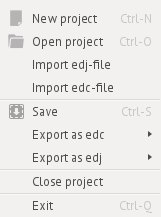
\includegraphics{images/file_menu.png}
Export as edc submenu

\includegraphics{images/file_export_as_edc_submenu.png}
User can export whole project to edc files tree or export only currently opened group into one single edc file and resource directories.
\subsubsection{View}
View section is provide ability to manipulate apperance of workspace area.
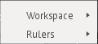
\includegraphics{images/view_menu.png}
Functionality of changing zoom fsctor or switching beetwen views on the workspace is placed in workspace submenu.
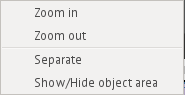
\includegraphics{images/view_workspace_submenu.png}
Manipulating rulers functions placed in rulers submenu
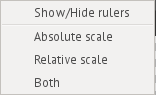
\includegraphics{images/view_rulers_submenu.png}
\chapter{Troubleshooting}
%Something like FAQ
\chapter{Appendix}
%Describe little thing like hotkeys, tips and examples
\end{document}